\chapter{热处理实验}
\section{TC4型钛合金的热处理工艺}
由~\ref{sec:1.1}可知,钛合金可以通过各种各样的相变过程来得到不同的组织结构。因而可以设计适宜的热处理工艺参数,来获得具有高强度的显微组织,由此实现\ti 合金力学性能和工艺性能的改善。\ti 合金热处理的一些特性如下:
\begin{enumerate}
%	\item 钛合金的热处理主要用于α+β型钛合金。因为对于纯α型钛合金而言,马氏体相变不会使钛合金的性能发生显著变化。只能依赖淬火形成的亚稳相(包括马氏体相)的时效分解来进行。
%	\item 热处理应该避免形成ω相。形成ω相会使钛合金变脆,正确选择时效工艺(例如,采用较高的时效温度)即可使相分解。
	\item α+β钛合金的淬透性差,淬火热应力大,淬火时零件易翘曲。由于导热性差,钛合金变形时易引起局部温升过高,使局部温度有可能超过β转变点而形成魏氏组织。
	\item 化学性质活泼。热处理时,钛合金易与氧和水蒸气反应,在工件表面形成具有一定深度的富氧层或氧化皮,使合金的性能降低。同时钛合金热处理时容易吸氢,引起氢脆。
	\item β转变点差异大。即使是同一成分,但由于冶炼炉次的不同,其β转变温度有时差别很大。
\end{enumerate}

常见的\ti 钛合金热处理工艺有:退火、淬火(往往加上时效处理)、形变热处理等,不同的热处理方式得到的组织性能各异。 鲁媛媛,马保飞等人研究发现在时效温度为450、500和550℃时初生α相的含量随温度升高逐渐增加;而在时效温度为600℃和650℃条件下初生α相含量因高温溶解而明显减少, β相尺寸相应增大。当时效温度为550℃时, 所得钛合金的显微组织最佳\cite{timing}。刘婉颖、林元华等人通过实验发现:在960 ℃/1 h + WQ进行固溶处理和500 ℃/4 h + AC下进行时效处理得到的\ti 具有最佳的力学性能\cite{960500};陈冠宇通过实验表明,在850℃进行退火处理时,在600℃进行时效处理可以使合金得到更好的耐腐蚀性能\cite{1200};李宸宇证明\ti 合金在900℃空冷固溶两小时在530℃时效四小时后具有更好的强硬度,而且固溶后冷速越快,合金的强硬度越高、塑韧性越差\cite{900}。%第46页


%不同热处理作用如下:
%\begin{enumerate}
%	\item 退火:用于提高合金塑形、稳定组织。
%	\item 淬火:用于强化组织,提高综合力学性能。
%	\item 形变热处理:与压力加工结合起来,同时发挥相变强化和热处理强化的作用。
%	\item 化学热强化:提高金属耐磨性,抗腐蚀性
%\end{enumerate}

%\subsection{热处理工艺对一般钛合金组织的影响}

\section{TC4钛合金的热处理方案设计}
对于α+β型的\ti 钛合金的固溶时效热处理工艺而言,其主要影响参数为温度和时间,在阅读了一些前人的研究报告\cite{mirror1}\cite{mirror2}之后,初步确定了固溶热处理的温度为950℃,本设计选择如下的参数来进行热处理操作,如表2.1所示\footnote{其中WQ表示水冷、FC表示炉冷、AC表示空冷。}
\begin{table}[htbp]
	\centering
	\label{sec:myHT}
	\caption{\ti 合金的热处理制度}
\begin{tabular}{cccccc}
	\toprule
		固溶温度/℃ &处理时间/h & 冷却方法 & 时效温度/℃  &处理时间/h & 冷却方法 \\
	\midrule
	910 & 1 & $\mathrm{WQ}$ & 510 & 4 & $\mathrm{AC}$\\
	910 & 1 & $\mathrm{FC}$  & 510 & 4 & $\mathrm{AC}$ \\
	910 & 1 & $\mathrm{WQ}$ & 550 & 4 & $\mathrm{AC}$ \\
	910 & 1 & $\mathrm{FC}$  & 550 & 4 & $\mathrm{AC}$ \\
	910 & 1 & $\mathrm{WQ}$ & 590 & 4 & $\mathrm{AC}$ \\
	910 & 1 & $\mathrm{FC}$  & 590 & 4 & $\mathrm{AC}$ \\
	\midrule
	950 & 1 & $\mathrm{WQ}$ & 510 & 4 & $\mathrm{AC}$ \\
	950 & 1 & $\mathrm{FC}$ & 510 & 4 & $\mathrm{AC}$ \\
	950 & 1 & $\mathrm{WQ}$ & 550 & 4 & $\mathrm{AC}$ \\
	950 & 1 & $\mathrm{FC}$ & 550 & 4 & $\mathrm{AC}$ \\
	950 & 1 & $\mathrm{WQ}$ & 590 & 4 & $\mathrm{AC}$ \\
	950 & 1 & $\mathrm{FC}$ & 590 & 4 & $\mathrm{AC}$ \\
	\midrule
	990 & 1 & $\mathrm{WQ}$ & 510 & 4 & $\mathrm{AC}$ \\
	990 & 1 & $\mathrm{FC}$ & 510 & 4 & $\mathrm{AC}$ \\
	990 & 1 & $\mathrm{WQ}$ & 550 & 4 & $\mathrm{AC}$ \\
	990 & 1 & $\mathrm{FC}$ & 550 & 4 & $\mathrm{AC}$ \\
	990 & 1 & $\mathrm{WQ}$ & 590 & 4 & $\mathrm{AC}$ \\
	990 & 1 & $\mathrm{FC}$ & 590 & 4 & $\mathrm{AC}$ \\
	\bottomrule
\end{tabular}
\end{table}
\section{TC4钛合金的热处理方案实验过程}
\subsection{实验材料}
实验用的是真空自耗两次熔炼所得的钛合金板,其化学成分参数与室温(20℃)力学性能参数如表2.2与表2.3所示:
\begin{table}[htbp]
	\centering
	\label{sec:mytc4chem}
	\caption{试样的化学成分参数}
	\begin{tabular}{ccccccccc}
		\toprule
	元素($ \% $) & Al & V &Fe &C& O& N &H &其他杂质\\ \midrule
	实际含量 & 6.12&4.06 &0.13 &0.012&0.112&0.009&0.004 &$ \le 0.4 $ \\
	标准要求 &$ 5.5\sim 6.75 $ & $ 3.5\sim 4.5 $&$ \le 0.30 $ & $ \le 0.05 $&$ \le 0.20 $&$ \le 0.03$ &$ \le 0.015 $  & -- \\ \bottomrule
	\end{tabular}
\end{table}

\begin{table}[htbp]
	\centering
	\label{sec:mytc4machin}
	\caption{试样的力学性能参数}
	\begin{tabular}{cccc}
		\toprule
		力学性能& 抗拉强度$Mpa  $& 屈服强度$ Mpa $&断后伸长率$ \% $\\ \midrule
		实测值 & 983 &902 & 13\\
		标准值 &$ \ge 895 $&$ \ge 830 $&$ \ge 10 $ \\ \bottomrule
	\end{tabular}
\end{table}


为了节约成本,本设计选择了尺寸较小的试样来进行实验,整体尺寸为$ 25mm\times 7.5mm $的狗骨状片体,具体参数如下图所示:
%3-28日上午,经过老师说明,由于试样为板材,加工成圆柱较为困难,故加工成二位平面的“狗骨头”

\begin{figure}[h!]
	\centering
	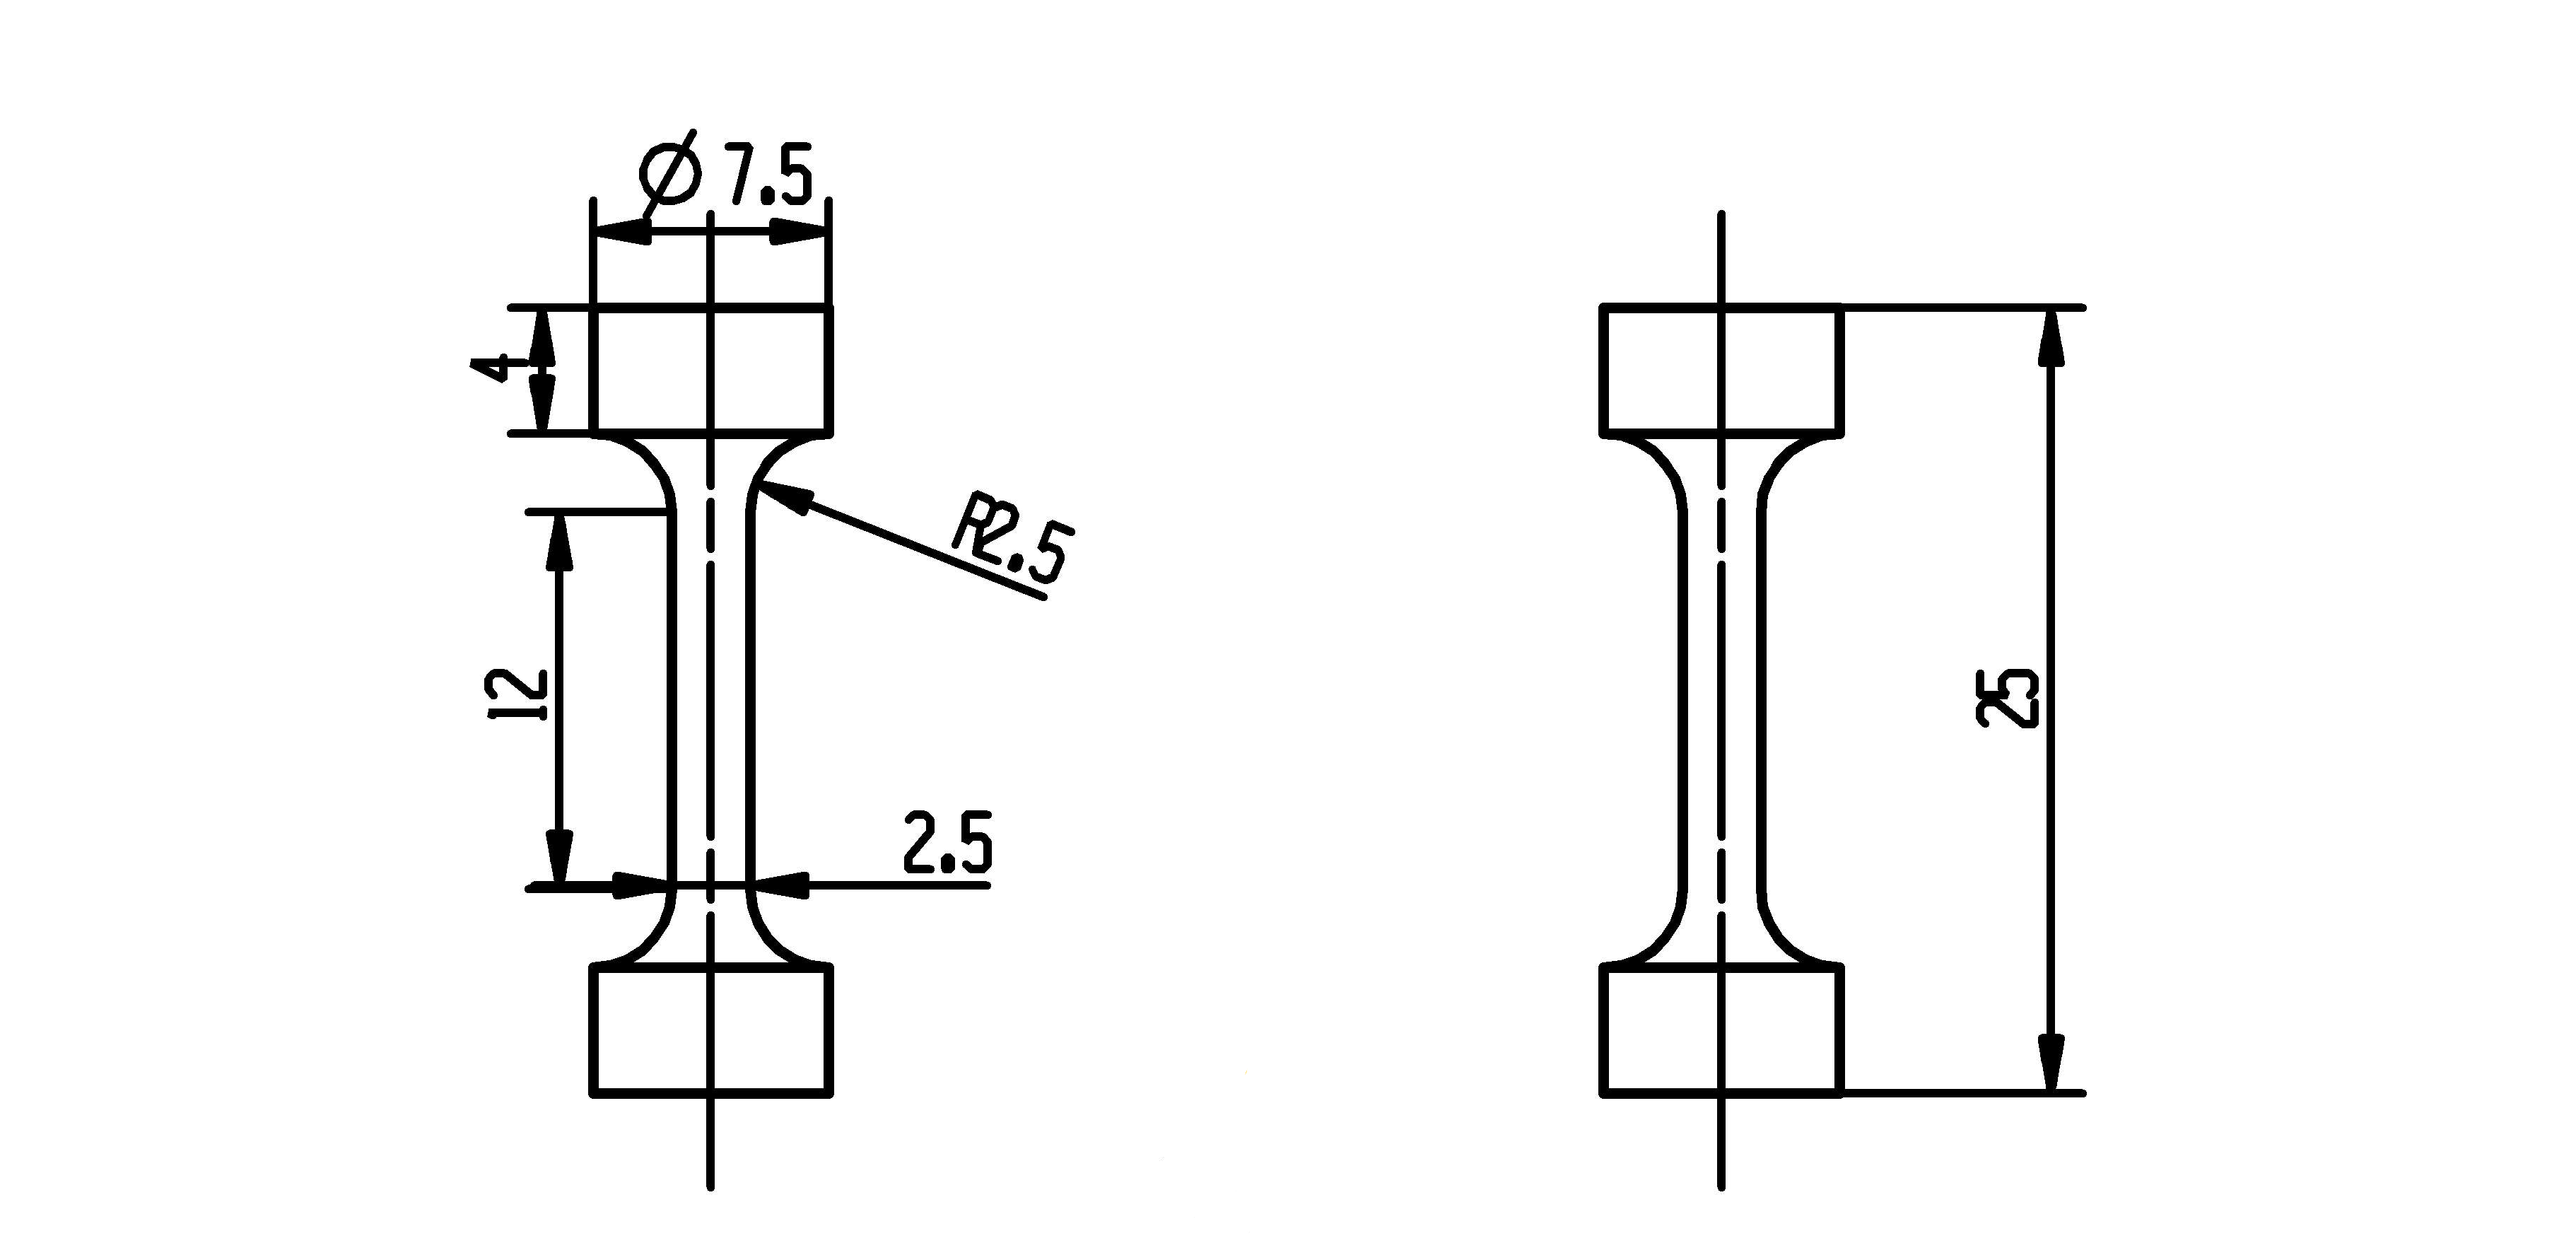
\includegraphics[width=0.99\linewidth]{pic/试样}
	\caption{试样的尺寸参数}
	\label{fig:试样尺寸}
\end{figure}

%
%\begin{figure}[!htbp]
%	\centering
%	\begin{minipage}[t]{0.68\textwidth}
%		\centering
%		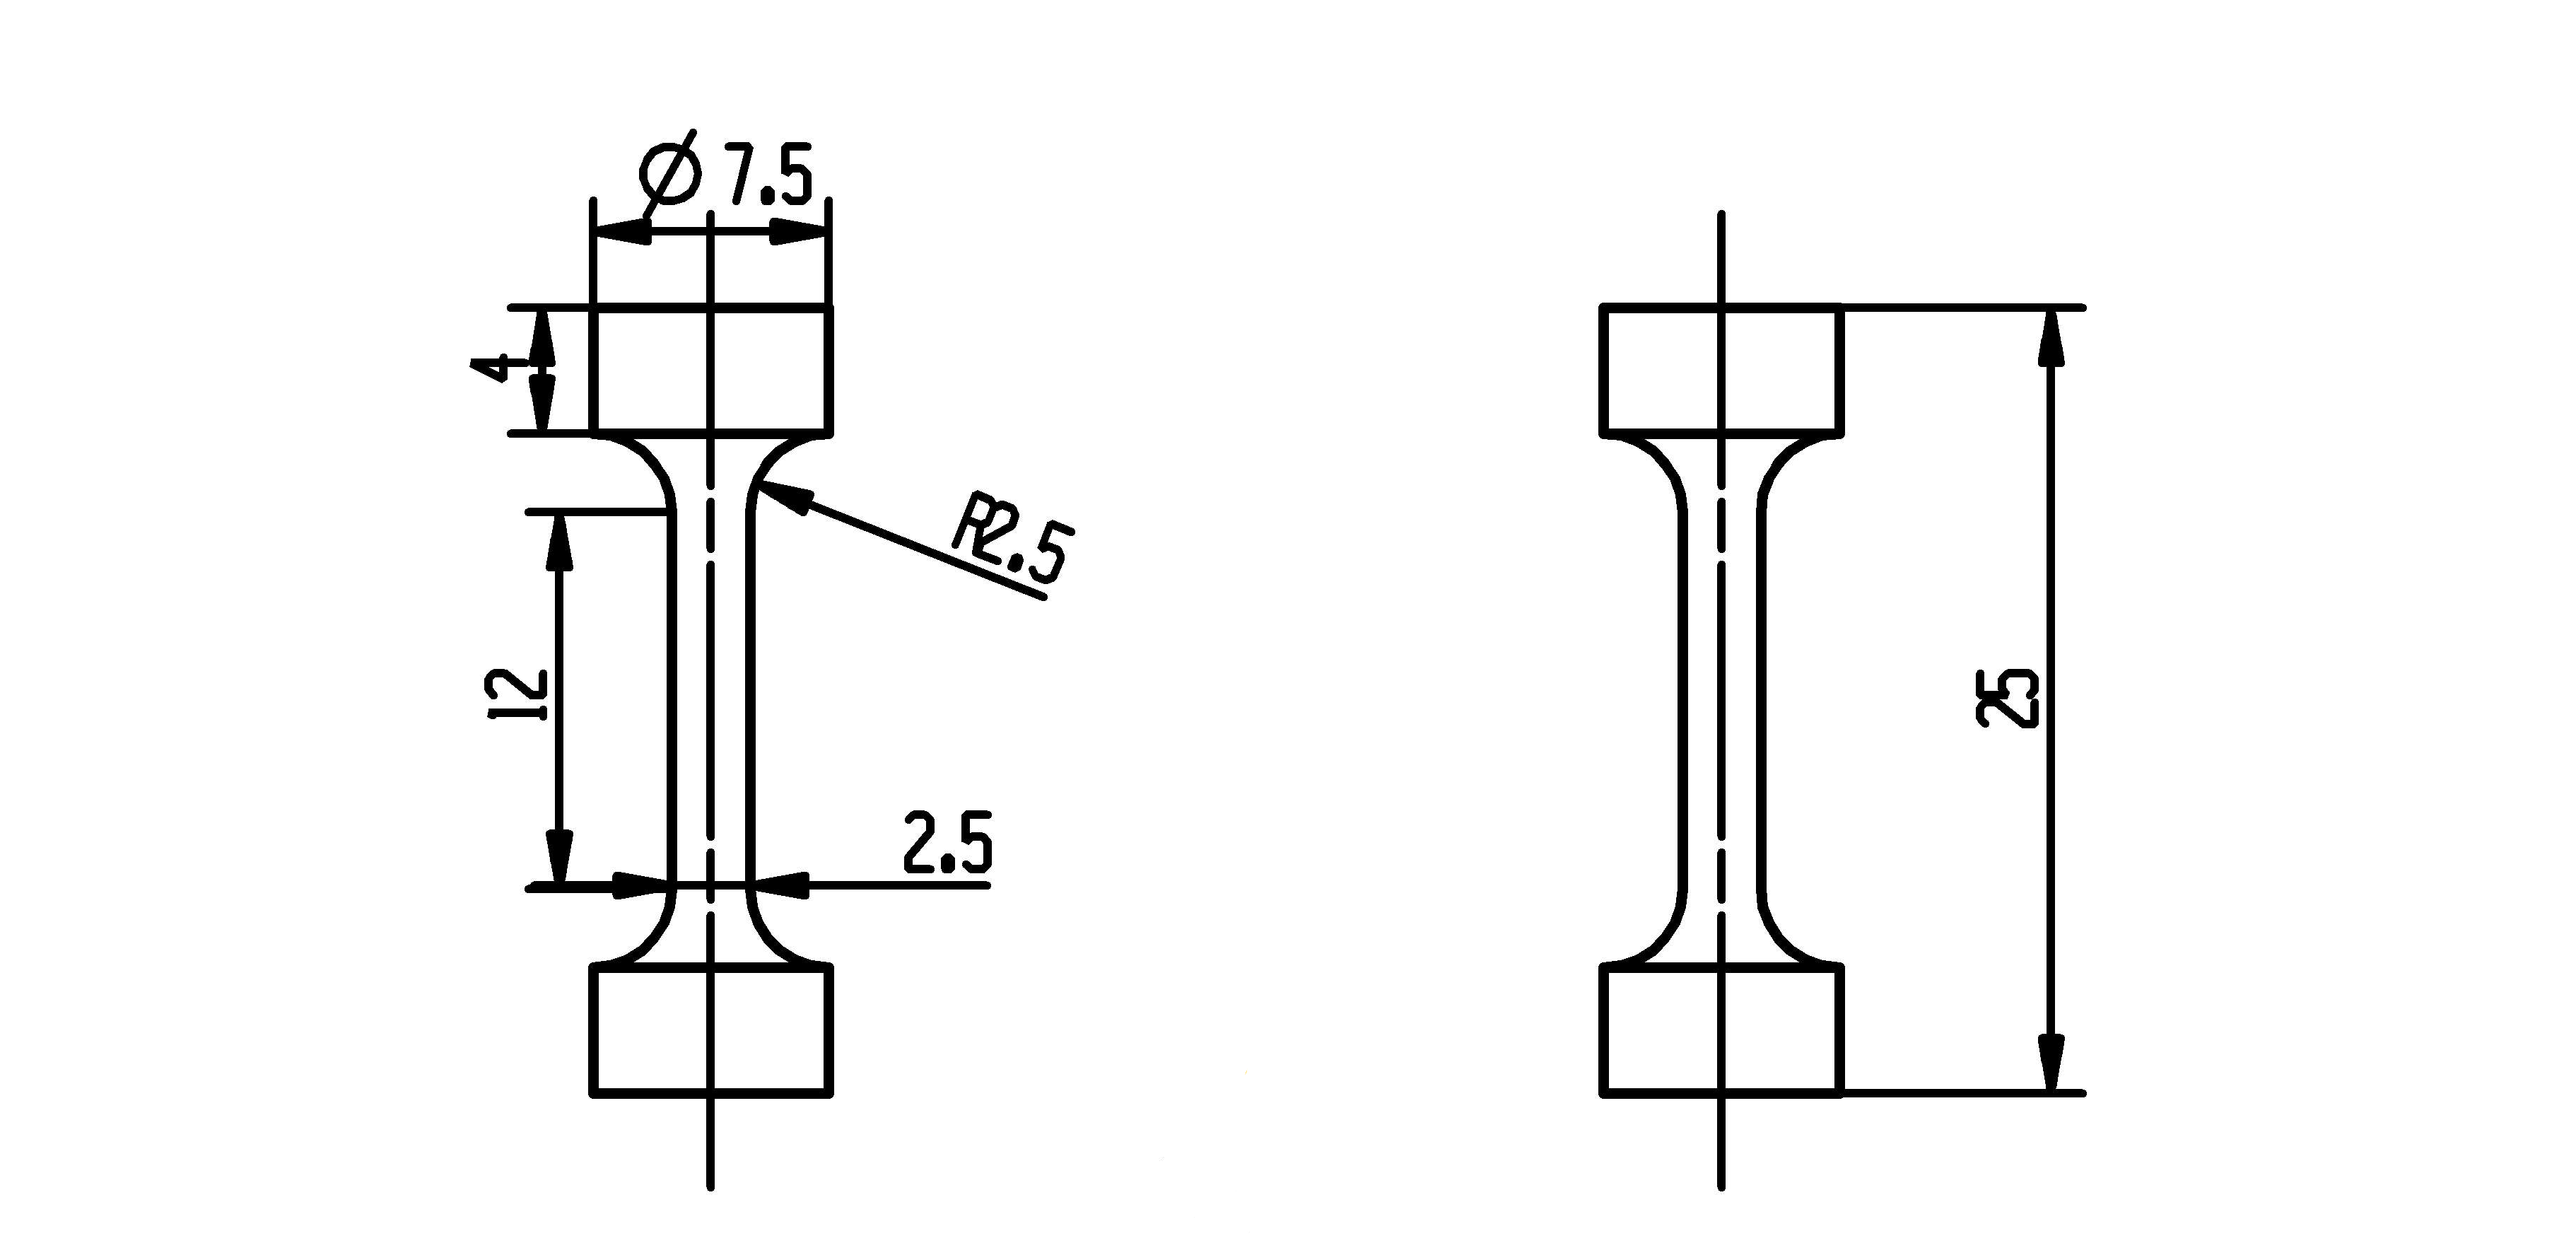
\includegraphics[width=6cm]{pic/试样}
%		\caption{试样的尺寸参数}
%		\label{fig:试样尺寸}
%	\end{minipage}
%	\begin{minipage}[t]{0.3\textwidth}
%		\centering
%		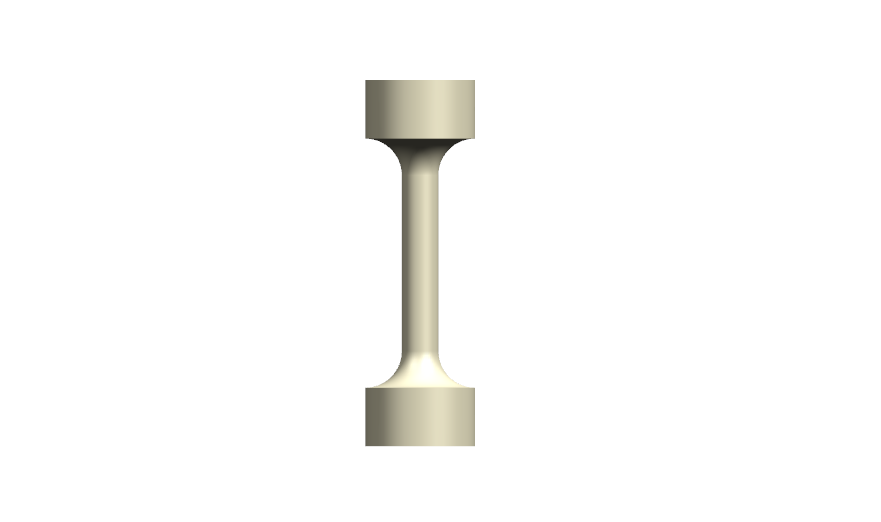
\includegraphics[width=6cm]{pic/模型}
%		\caption{试样的三维模型}
%		\label{fig:试样的三维模型}
%	\end{minipage}
%%	\caption{试样参数}
%\end{figure}

\subsection{实验过程}


\section{小结}
